\documentclass{beamer}  
%导言区
%\usepackage[UTF8,noindent]{ctexcap}%阻止ctex宏包引入的短浅缩进
\usetheme{AnnArbor}
\usepackage{graphicx}
%set equation theme
\setbeamertemplate{footline}[frame number]{}
\usefonttheme{professionalfonts}
\usepackage{algorithm2e}
\usepackage{algorithmic}
\usepackage[level]{datetime} 



%set theme
\useinnertheme{rectangles}
\useoutertheme{smoothbars}%sidebar
\usecolortheme{crane}%crane
\begin{document}  
	
%second section 
	
	
	\title[WGAN]{High-Resolution Image Synthesis and Semantic Manipulation with Conditional GANs}
	\institute[SCUT]{South China University of Technology}
	%\logo{
\includegraphics[height=0.45\textwidth]{graphics/scut.pdf}}
	\author{Presented by Junhong Huang}
	\titlegraphic{	
\includegraphics[height=0.35\textwidth]{images/scut.pdf}}
	\date{May 20, 2018, SAIL}
	\keywords{GAN,WGAN,machine learning,deep learning}
	
	%first
	\begin{frame}
	\maketitle
\end{frame}

\begin{frame}{Contents}
%content
\tableofcontents
\end{frame}



\AtBeginSection[]
{
\begin{frame}{Contents}

\tableofcontents[currentsection]

\end{frame}
}

\section{Motivation}
\begin{frame}
\begin{figure}
	\centering
	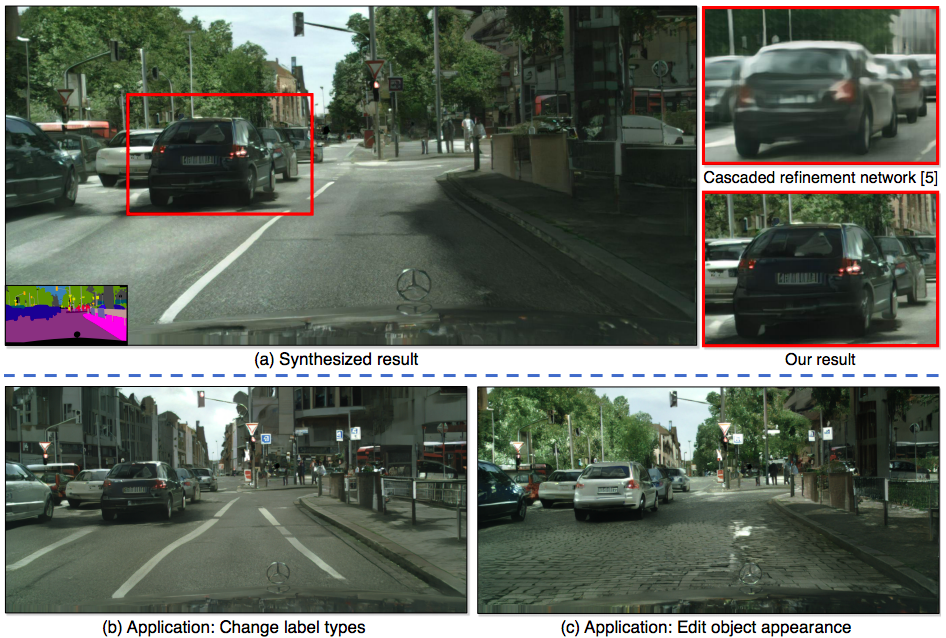
\includegraphics[height=0.45\textheight]{images/conclusion}
\end{figure}
\end{frame}

\section{Method}
\begin{frame}
	\begin{figure}
	\centering
	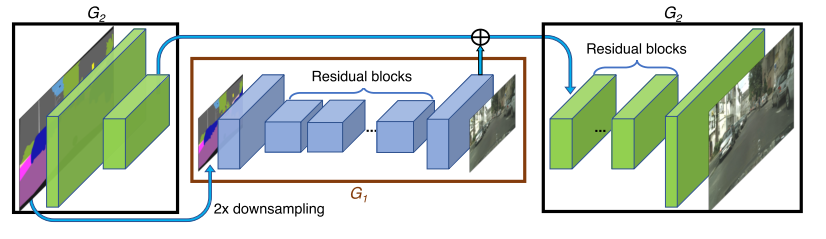
\includegraphics[height=0.45\textheight]{images/structure}
\end{figure}
\end{frame}

\begin{frame}
\begin{figure}
	\centering
	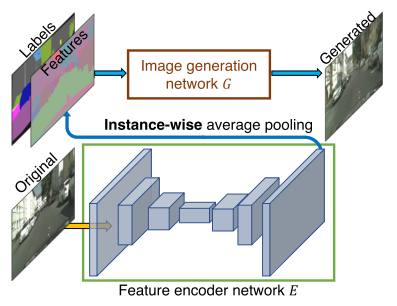
\includegraphics[height=0.45\textheight]{images/instance}
\end{figure}

\begin{figure}
	\centering
	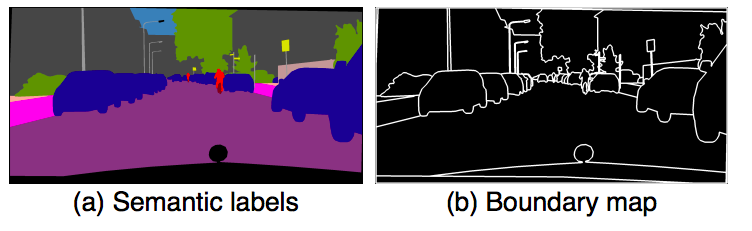
\includegraphics[height=0.45\textheight]{images/instance_maps}
\end{figure}
\end{frame}

\begin{frame}
\begin{figure}
	\centering
	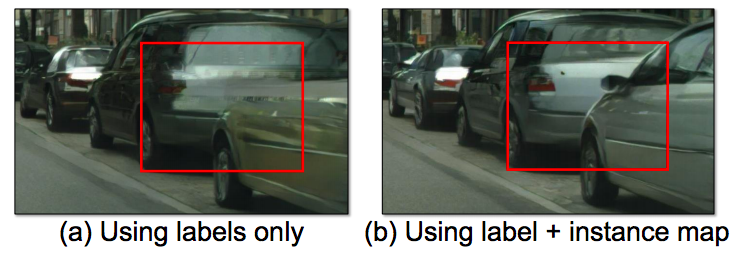
\includegraphics[height=0.45\textheight]{images/instance_result}
\end{figure}
\end{frame}

\begin{frame}
\begin{figure}
	\centering
	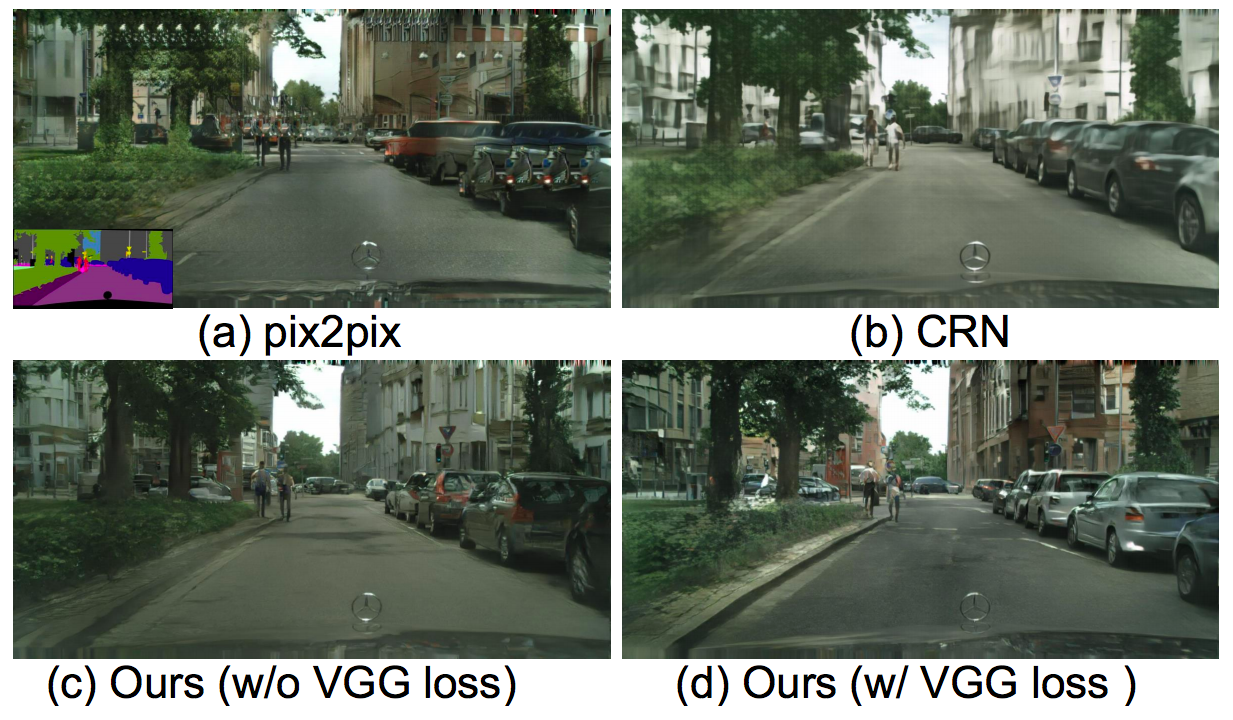
\includegraphics[height=0.45\textheight]{images/result_1}
\end{figure}
\end{frame}

\begin{frame}
\begin{figure}
	\centering
	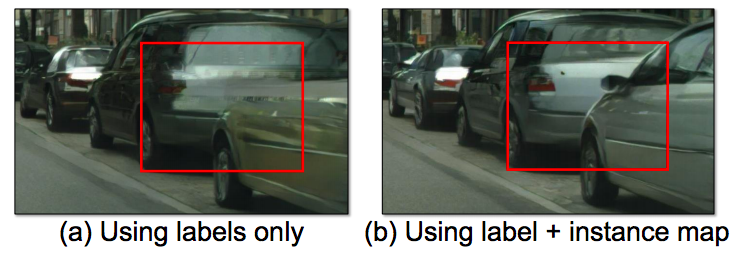
\includegraphics[height=0.45\textheight]{images/instance_result}
\end{figure}
\end{frame}

\section{Experimental Results}

\begin{frame}
\begin{figure}
	\centering
	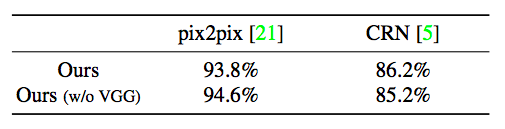
\includegraphics[height=0.35\textheight]{images/unlimite_time}
\end{figure}
\end{frame}

\begin{frame}
\begin{figure}
	\centering
	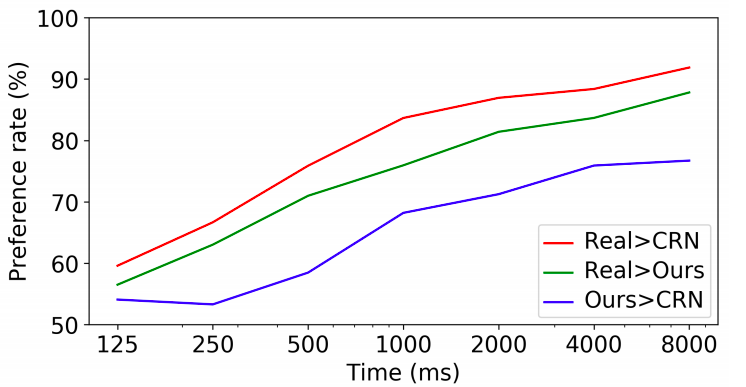
\includegraphics[height=0.45\textheight]{images/limite_time}
\end{figure}
\end{frame}

\begin{frame}
\begin{figure}
	\centering
	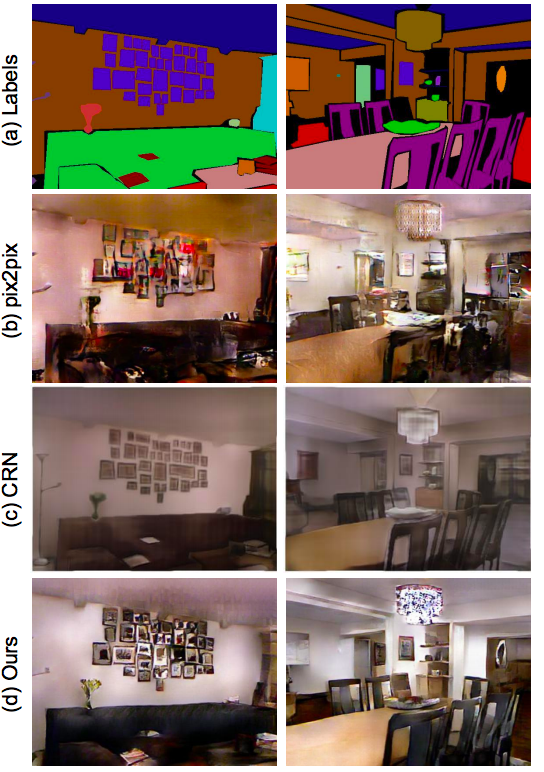
\includegraphics[height=0.45\textheight]{images/result_2}
\end{figure}
\end{frame}

\begin{frame}
\begin{figure}
	\centering
	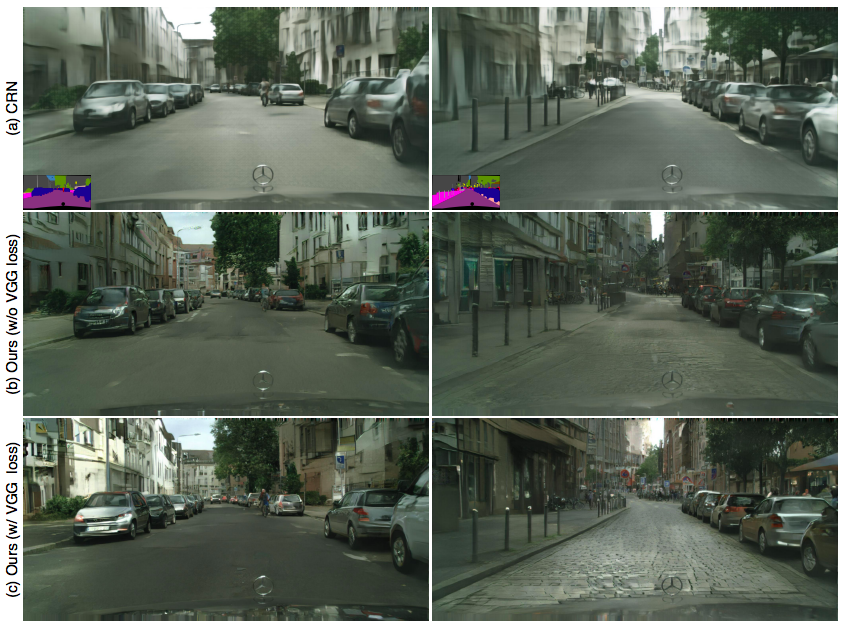
\includegraphics[height=0.45\textheight]{images/result_3}
\end{figure}
\end{frame}

\begin{frame}
\begin{figure}
	\centering
	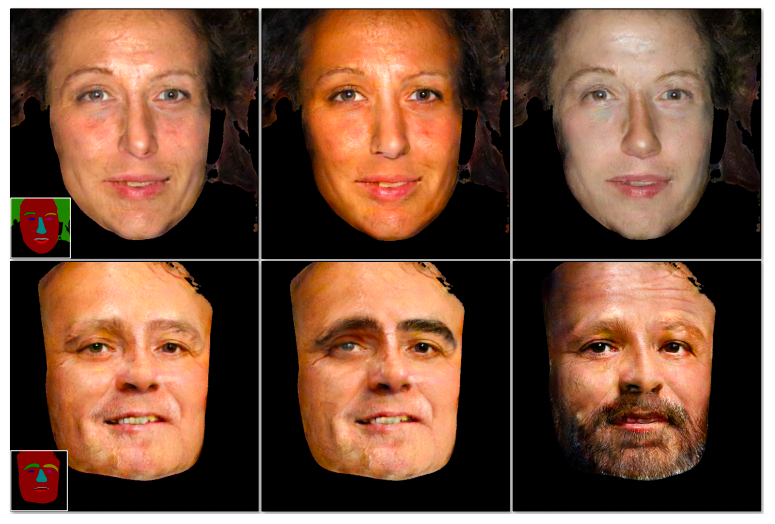
\includegraphics[height=0.45\textheight]{images/result_4}
\end{figure}
\end{frame}

\section{Conclusions}

\end{document} 